\AdvanceDate[0]

\pagestyle{fancy}
\fancyhead[L]{Seconde 13}
\fancyhead[C]{\textbf{Probabilités 2 \ifsolutions -- Solutions  \fi}}
\fancyhead[R]{\today}

\exe{	
	On tire un boule dans une urne contenant $2$ boules rouges et $4$ boules vertes.
	\begin{enumerate}[label=$\bullet$]
		\item Si la boule tirée est verte, on la met de côté et on retire une nouvelle boule
		\item Si la boule tirée est rouge, on la remet dans l'urne et on retire une nouvelle boule
	\end{enumerate}
	On distingue les quatre événements suivants :
		\begin{multicols}{2}
		\begin{enumerate}[label=]
			\item v : \og la première boule tirée est verte \fg
			\item r : \og la première boule tirée est rouge \fg
			\item V : \og la deuxième boule tirée est verte \fg
			\item R : \og la deuxième boule tirée est rouge \fg
		\end{enumerate}
		\end{multicols}
	\begin{center}
	\begin{tikzpicture}
		% depth 1
		\foreach \i in {-3, 3}
		\draw[-, thick, black] (0,0) node {$\bullet$} -- (\i,-2);
		% depth 2
		\foreach \i in {-3, 3} \foreach \j in {-1, 1}
			\draw[-, thick, black] (\i,-2) node {$\bullet$} -- (\i+\j,-4) node {$\bullet$};
			
		\draw (-3,-2) node[above left] {$v$};
		\draw (3,-2) node[above right] {$r$};
			
		\draw (-4,-4) node[below] {$V$};
		\draw (2,-4) node[below] {$V$};
		\draw (-2,-4) node[below] {$R$};
		\draw (4,-4) node[below] {$R$};
	\end{tikzpicture}
	\end{center}
	Compléter l'arbre, calculer $P(V)$ et $P(R)$.
}{}

\exe{
	Compléter l'arbre correspondant à une expérience aléatoire à deux épreuves d'univers $\{A ; B ; C ; D\}$ et répondre aux questions suivantes.
	\begin{center}
	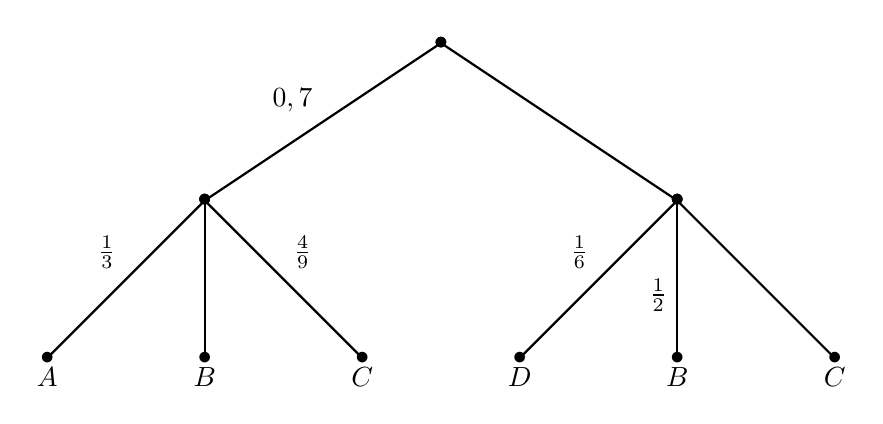
\begin{tikzpicture}
		% depth 1
		\draw[-, thick, black] (0,0) node {$\bullet$} -- (3,-2) node[midway, above right] {};
		\draw[-, thick, black] (0,0) node {$\bullet$} -- (-3,-2) node[midway, above left] {$0,7$};
		% depth 2
		\draw[-, thick, black] (-3,-2) node {$\bullet$} -- (-1,-4) node[midway, above right] {$\frac49$};
		\draw[-, thick, black] (-3,-2) node {$\bullet$} -- (-3,-4);
		\draw[-, thick, black] (-3,-2) node {$\bullet$} -- (-5,-4) node[midway, above left] {$\frac13$};
		
		\draw[-, thick, black] (3,-2) node {$\bullet$} -- (1,-4) node[midway, above left] {$\frac16$};
		\draw[-, thick, black] (3,-2) node {$\bullet$} -- (3,-4) node[pos=.6, left] {$\frac12$};
		\draw[-, thick, black] (3,-2) node {$\bullet$} -- (5,-4);
		
		\draw (1,-4) node {$\bullet$};
		\draw (3,-4) node {$\bullet$};
		\draw (5,-4) node {$\bullet$};
		\draw (1,-4) node[below] {$D$};
		\draw (3,-4) node[below] {$B$};
		\draw (5,-4) node[below] {$C$};
		
		\draw (-1,-4) node {$\bullet$};
		\draw (-3,-4) node {$\bullet$};
		\draw (-5,-4) node {$\bullet$};
		\draw (-1,-4) node[below] {$C$};
		\draw (-3,-4) node[below] {$B$};
		\draw (-5,-4) node[below] {$A$};
	\end{tikzpicture}
	\end{center}
	
	\begin{multicols}{2}
	\begin{enumerate}
		\item Calculer $P(D)$.
		\item Calculer $P(B)$.
		\item Calculer $P(D \cup B)$.
		\item Calculer $P(A\cup C)$.
	\end{enumerate}
	\end{multicols}

}{}

\newpage

\exe{
	On tire un boule dans une urne contenant $3$ boules bleues et $4$ boules vertes.
	\begin{enumerate}[label=$\bullet$]
		\item Si la boule tirée est verte, on jette un dé équilibré à $3$ faces
		\item Si la boule tirée est rouge, on jette un dé équilibré à $6$ faces
	\end{enumerate}

	Créer un arbre de probabilité pour cette situation et répondre aux questions suivantes.
	\begin{enumerate}
		\item Quelle est la probabilité d'obtenir un nombre pair ?
		\item Quelle est la probabilité d'obtenir un multiple de $3$ ?
		\item Quelle est la probabilité d'obtenir un nombre pair \textbf{ou} un multiple de $3$ ?
		\item Calculer la probabilité d'obtenir $6$ et vérifier la formule d'inclusion-exclusion.
	\end{enumerate}

}{}

\exe{	
	Dans une urne opaque se trouvent un nombre inconnu de boules rouges, bleues, et vertes.
	On tire aléatoirement une boule de l'urne, on note sa couleur, et on la remet dans l'urne.
	Les résultats sont décrits dans le tableau suivant.
	\begin{center}
	\begin{tabular}{|c|c|c|c|} \hline
		Couleur & Rouge & Bleu & Vert \\ \hline
		Nombre de tirages & \rouge & \bleu & \vert \\ \hline
		Fréquence & & & \\ \hline
	\end{tabular}
	\end{center}
	
	Compléter le tableau, modéliser la réalité en définissant un univers et une loi de probabilité, et l'utiliser pour répondre aux questions suivantes.
	\begin{enumerate}
		\item Quelle est la probabilité d'obtenir deux boules rouges en deux tirages ?
		\item Quelle est la probabilité d'obtenir deux boules vertes en trois tirages ?
		\item Quelle est la probabilité d'obtenir au moins une boule bleue en quatre tirages ?
	\end{enumerate}
}{}

\exe{	
	On lancer un grand nombre de fois un D$6$, dé à $6$ faces.
	Les résultats sont décrits dans le tableau suivant.
	\begin{center}
	\begin{tabular}{|c|c|c|c|c|c|c|} \hline
		Face & 1 & 2 & 3 & 4 & 5 & 6 \\ \hline
		Nombre de tirages & \un & \deux & \trois & \quatre & \cinq & \six \\ \hline
		Fréquence & & & & & &\\ \hline
	\end{tabular}
	\end{center}
	
	Compléter le tableau, modéliser la réalité en définissant un univers et une loi de probabilité, et l'utiliser pour répondre aux questions suivantes.
	\begin{enumerate}
		\item Quelle est la probabilité d'obtenir un nombre pair ?
		\item Quelle est la probabilité d'obtenir deux $6$ en deux lancers consécutifs ?
		\item Quelle est la probabilité d'obtenir au moins un $6$ après $4$ lancers ?
	\end{enumerate}
}{}

\end{document}
